\section{Benchmarks}
\label{sec-benchmarks}

We implemented ten different versions of \texttt{reverse-count}, a
function that counts elements of a list from the end.  The difference
between these versions can be expressed in terms of two different
numeric parameters, namely:

\begin{enumerate}
\item the minimum number of elements for which we apply the
  logarithmic method, consisting of dividing the list into two
  equal-size halves, and
\item into how many chunks do we cut the list when the number of
  elements is smaller than the first parameter, but larger than the
  number of elements that can be handled by the simple recursive
  technique.
\end{enumerate}

In all of our versions, when the number of elements is less than
$10000$, we process the elements using the purely recursive technique
where the element is processed in the backtracking phase.

For the purpose of this article,
we have retained the one with the best experimental behavior (\texttt{v7})
and compared it to two more traditional versions  (\texttt{v0} and \texttt{v1}).

These three versions can be characterized as follows:

\begin{enumerate}
\setcounter{enumi}{-1}
\item Version \texttt{v0} uses the native \texttt{count} function
  called with the \texttt{from-end} keyword argument set to
  \texttt{t},
\verbatimtabinput{Code/Count/0-count.lisp}
\item Version \texttt{v1} is the naive version consisting in reversing the list 
before counting; this version uses the heap space and no stack space.
\verbatimtabinput{Code/Count/1-count.lisp}
\setcounter{enumi}{6}
\item Version \texttt{v7} divides the list in 2 parts
if it has more than one 
hundred million elements.  Otherwise, if it has more than 10000
elements, it divides it into chunks that have 10000 elements each.
Finally, if it has no more than 10000 elements, then it uses the
standard recursive method.

We think this method is faster than the others, at least for
lengths no more than one hundred million elements, because then it
is guaranteed to traverse the list at most 3 times + 1 time for
computing the length.  It could be improved for lengths greater
than one hundred million by using a better division than 2 in this
case, but we have not attempted that improvement.
The code is given below.
\end{enumerate}

\verbatimtabinput{Code/Count/7-count.lisp}

Thanks to the help of the Lisp community, we could test the behavior
of these three versions on several implementations and architectures.
In \refFig{f-systems}, we summarize the results of tests that worked
for a list of size up to $10^7$.  In many cases, the details of the
implementation are unknown or not shown.  However, the purpose of the
\refFig{f-systems} is not to compare performance between different
systems, but to compare the performance of different versions of
\texttt{count} on each system.  For that reason, the exact details of
the system are unimportant; we are only interested in whether
\texttt{v7} compares favorably to the other versions on most systems.
Furthermore, for some implementations, we had to change the
\texttt{optimize} settings and some other parameters in order to get
our code to work.%
\footnote{In particular, \lispworks{} has a much smaller default stack
  than for instance \sbcl{} (16k words, compared to 250k words)
  resulting in stack overflow of our benchmark with default
  parameters.  For that reason, we ran the \lispworks{} benchmark with
  a smaller stack and with a higher value of \texttt{safety}.  The
  combination of these factors is the likely explanation to the
  absence of performance improvement for \lispworks{}.  However, we
  are told that on 32-bit \lispworks{} our technique gives a factor
  $10$ improvement.}  For that reason, it is not possible to compare
the performance on different implementations in \refFig{f-systems},
even when the processor and the clock frequency are the same.

\begin{figure*}[htb]
\centering
\begin{tabular}{|c|c|c|c|c|c|c|}
\hline
\multicolumn{4}{|c|}{System characteristics}  & \multicolumn{3}{|c|}{Time in seconds}\\ \hline
Implementation & Version      & Processor                  & Frequency          & v0 & v1 & v7 \\ \hline
LispWorks  & 6.1.1            & Intel Core &  ?                 & 0.20 & 0.18 & 0.14 \\ \hline
Clozure CL & 1.10     & Intel Xeon & 3.33GHz            & 1.93 & 1.79 & 0.15 \\ \hline
Clozure CL & 1.10-dev & AMD FX & ? & 1.77 & 1.63 & 0.15 \\ \hline
SBCL       & 1.2.8 & Intel Xeon & 3.33GHz            & 0.51 & 0.27 & 0.22 \\ \hline
ABCL       & 1.3.1            & Intel Xeon & 3.33GHz            & 1.13 & 0.22 & 0.34 \\ \hline
CLISP      & 2.49             & X86\_64                    &   ?                & 1.15 & 1.14 & 0.87 \\ \hline
ECL        & 13.5.1           & ?                          &   ?                & 0.69 & 0.41 & 0.36 \\ \hline
SBCL       & 1.2.7 & Intel Core & 2.53GHz      & 0.36 & 0.38 & 0.25 \\ \hline
\end{tabular}
\caption{\label{f-systems} Performances of the three versions on several systems with a list of $10^7$ elements}
\end{figure*}

To get a better idea of the difference in performance between the
three versions of the \texttt{count} function, we selected the table
entry corresponding to the non-commercial implementation that resulted
in the greatest advantage of our \texttt{v7} compared to the other
versions (\texttt{Clozure CL 1.10-dev}), and we rendered the
performance in the form of a graph.  The result is shown in
\refFig{f-versions}.

\begin{figure*}[htb]
\centering
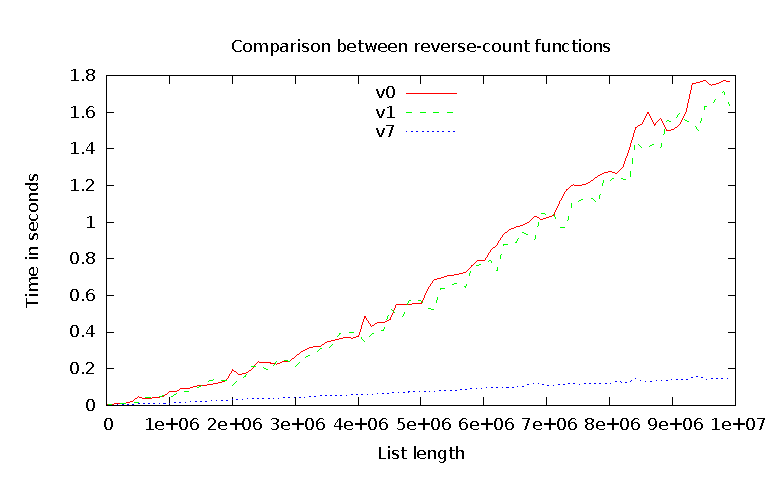
\includegraphics{v0-v1-v7.eps}
\caption{\label{f-versions} Comparison of the behavior of the three versions on a single system}
\end{figure*}

As \refFig{f-versions} shows, the performance of \texttt{v7} is
significantly better than that of the other versions.  Furthermore,
the fact that the curve for \texttt{v7} is smoother than the curves
for other versions indicates that the performance of \texttt{v7} is
more predictable.  We attribute this behavior to the garbage
collector, which occasionally has to run when heap allocation is
required.  Since \texttt{v7} does not require any heap allocation, the
garbage collector is not solicited.

%%  LocalWords:  
